
\section{Signal Separation using Non Negative Matrix Factorization}

In this problem you will use NMF to separate a mixed signal into its component signals. Specifically, your goal is to separate music and speech sounds from a signal consisting of both.

The basic idea is that you will use NMF to first learn bases for speech and music. Then you will use the learned bases to separate out music and speech from a recording consisting of both.

Do the following processing steps.
\begin{enumerate}
    \item  In the directory \texttt{hw2materials/problem3} you will find \texttt{speech.wav} file. Read the speech signal and compute its spectrogram. You already did this in previous homework 1. Use the \texttt{stft} function followed by magnitude computation, as before;  
    \begin{lstlisting}
    [s, fs] = audioread('filename');
    spectrogram = stft(s',2048,256,0,hann(2048))
    M = abs(spectrogram)
    \end{lstlisting}
    
    \item Do the same for \texttt{music.wav} file.
\end{enumerate}
If we call $M_m$ and $M_s$ the magnitude spectrum of the music and speech file respectively, then the dimensionality of both matrices should be $1025 \times 977$. 

\begin{figure}[h!]
    \centering
    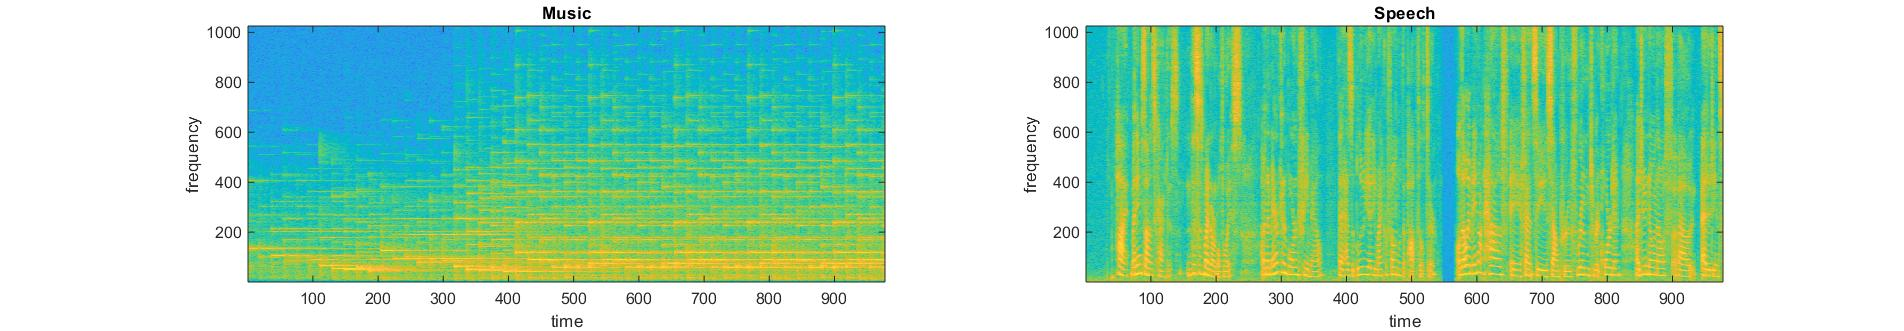
\includegraphics[trim ={6cm 0 0 0 }, scale=0.3]{figs/music_speech.jpg}
    \caption{Magnitude spectrum (in log scale) of files \texttt{music.wav} and \texttt{speech.wav}}
    \label{face_example}
\end{figure}


Now using the spectrograms for music $M_m$ and speech $M_s$ you are first going to learn bases, $B_m$ and $B_s$ for music and speech respectively. Therefore, given the non-negative matrices $M_m$ and $M_s$, we need to find the non-negative matrices $B_m$, $W_m$, $B_s$ and $W_s$ such that
\begin{eqnarray}
    M_m & \approx & B_m \, W_m\\
    M_s & \approx & B_s \, \, W_s
\end{eqnarray}

 
\subsection{NMF Estimation: Learning Bases}

In this homework, given a non-negative matrix $M \in \mathbb{R}^{p \times q}$, we will consider the algorithm to estimate the non-negative matrices $B \in \mathbb{R}^{p \times k}$ and $W \in \mathbb{R}^{k \times q}$ that attempts to minimize the \textit{KL divergence} between $M$ and $BW$. The KL divergence between matrix $A$ and matrix $B$ is given by
\begin{eqnarray}
        D(A \,  || \, B) & = & \sum_{ij} \left( A_{ij} \log \left( \frac{A_{ij}}{B_{ij}} \right) - A_{ij} + B_{ij} \right) 
    \end{eqnarray}
Then, the algorithm that minimizes $D(M || BW)$ is the following:
\begin{itemize}
    \item Initialize $B$ and $W$ randomly.
    \item Iteratively update $B$ and $W$ using the following rule:
    \begin{eqnarray}
        B = B \, \otimes \, \frac{\left( \frac{M}{BW} \right) W^\top}{{\bf 1}_{p \times q} W^\top} \\
        W = W \, \otimes \, \frac{B^\top \left( \frac{M}{BW} \right)}{B^\top {\bf 1}_{p \times q}}
    \end{eqnarray}
    where $\otimes$ denotes component-wise matrix multiplication, $\frac{\; \cdot \;}{\cdot}$ denotes the component-wise matrix division, and ${\bf 1}_{p \times q}$ is the $p \times q$ matrix which each of its component is 1.
\end{itemize}

\begin{enumerate}
    \item Write the function \texttt{NMF\_train} which receives as inputs:
    \begin{itemize}
        \item \texttt{M}: a $p \times q$ non-negative matrix. 
        \item \texttt{B\_init}:  a $p \times k$ non-negative matrix. This matrix is the initial value of matrix $B$.
        \item \texttt{W\_init}: a $k \times q$ non-negative matrix. This matrix is the initial value of matrix $W$.
        \item \texttt{n\_iter}: a positive integer value. It determines the number of iterations of the algorithm.
    \end{itemize}
    Based on the algorithm previously described, the outputs of this function must be:
    \begin{itemize}
        \item \texttt{B}: a $p \times k$ non-negative matrix. 
        \item \texttt{W}: a $k \times q$ non-negative matrix.
    \end{itemize}
    \ul{Submit your code.}
    
    \item In the directory \texttt{hw2materials/problem3} you can find the files \texttt{Bm\_init.csv} and \texttt{Wm\_init.csv}. These files are matrices which must be used as initial condition to run your function \texttt{NMF\_train} over the magnitude spectrum of the music signal $M_m$. Consider values for \texttt{n\_iter} in $\{0, 50, 100, 150, 200, 250\}$. Run your function using these parameters and plot $D(M_m || B_mW_m)$ as function of \texttt{n\_iter}. \ul{Attach this plot to your report and write the value of $D(M_m||B_mW_m)$ for \texttt{n\_iter} $= 250$}.
    
    \item Similarly, you can also find in the directory \texttt{hw2materials/problem3} the files \texttt{Bs\_init.csv} and \texttt{Ws\_init.csv}. As before, these files are matrices which must be used as initial condition to run your function \texttt{NMF\_train} over the magnitude spectrum of the speech signal $M_s$. Repeat the previous task your this signal considering the same setting. \ul{Attach your plot to the report and write the value of $D(M_s||B_sW_s)$ for \texttt{n\_iter} $= 250$}. 
    
\end{enumerate}


\subsection{Signal Separation}

Now, using the bases you learned for speech and music, we will separate a signal which is a mix between a different speech signal and a music signal.

In the directory \texttt{hw2materials/problem3} you can find a file named \texttt{mixed.wav}. Compute its magnitude spectrum, that we will call $M_{\text{mixed}}$. The following figure visualize this matrix.

\begin{figure}[h!]
    \centering
    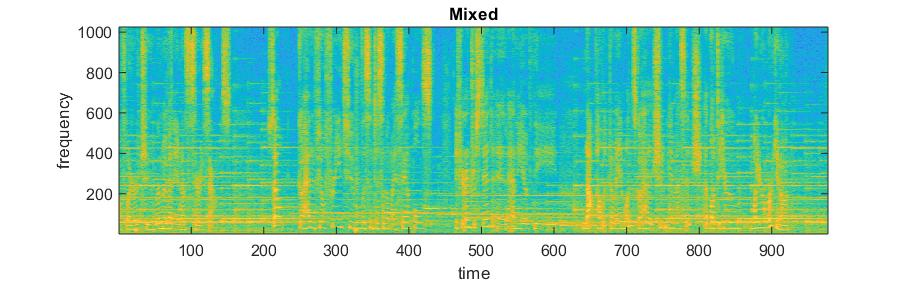
\includegraphics[trim ={0cm 0 0 0 }, scale=0.3]{figs/mixed.jpg}
    \caption{Magnitude spectrum (in log scale) of file \texttt{mixed.wav}}
\end{figure}



Our model considers that the bases we learned in the previous part are good enough to represent this audio file. More precisely, in this case, given $M_{\text{mixed}}$, $B_s$ and $B_m$, we need to learn the weights $W$ such that
\begin{eqnarray}
    M_{\text{mixed}} & \approx & [B_s \; B_m] W 
\end{eqnarray}
 In this equation, $[B_s \; B_m]$ represents the concatenation of the bases you already learned; so if $M_{\text{mixed}}$ is a $p \times q$ matrix, $[B_s \; B_m]$ is a $p \times 2k$ matrix. Moreover, the matrix $W$ gives us the contribution of each element in this \textit{new} set of bases. 
 To learn $W$ we can use the previous algorithm, but without updating the bases $B$ (we already know $B$).
 

\begin{enumerate}
    \item Write the function \texttt{separate\_signals} which receives as inputs:
    \begin{itemize}
        \item \texttt{M\_mixed}: a $p \times q$ non-negative matrix. 
        \item \texttt{B\_speech}:  a $p \times k$ non-negative matrix. This matrix is the bases you have to represent speech.
        \item \texttt{B\_music}: a $p \times k$ non-negative matrix. This matrix is the bases you have to represent music.
        \item \texttt{n\_iter}: a positive integer value. It determines the number of iterations of the algorithm.
    \end{itemize}
    The output of this function must be:
    \begin{itemize}
        \item \texttt{M\_speech\_rec}: a $p \times q$ non-negative matrix. It is the recovered speech magnitude spectrum.
        \item \texttt{M\_music\_rec}: a $p \times q$ non-negative matrix. It is the recovered music magnitude spectrum.
    \end{itemize}
    \ul{Submit your code}
    
    \item Using the bases you learned from the previous problem when you considered \texttt{n\_iter} $= 250$, apply your function \texttt{separate\_signals} using the magnitude spectrum of the mixed signal and taking \texttt{n\_iter} = 500. \ul{Submit your output as \texttt{M\_speech\_rec.csv} and \texttt{M\_music\_rec.csv}}.
    
    
    \item Now using the phase for the mixed signal along with reconstructed spectrograms, reconstruct time domain music and speech signals. You did this in homework 1 as well. You can use the \texttt{stft} function again to do this. Save the generated signals as \texttt{speech\_rec.wav} and \texttt{music\_rec.wav}. \ul{Submit these two files}.
    
    
\end{enumerate}